\subsubsection{Modelado del mapa}

Para empezar, es crucial tener un diseño inicial del entorno donde se moverá el robot, que incluya paredes, obstáculos y puntos de interés. Dado que el robot solo se mueve en líneas rectas, este proceso puede ser más sencillo en comparación con robots que tienen libertad de movimiento en todas las direcciones.

El siguiente paso fue la creación del modelo del mapa, donde se divide el entorno en una cuadrícula (grid) y cada celda se marca como libre, ocupada, obstáculo o borde. Cada celda es cuadrada y tiene un lado de $0.5[m]$. Además de ello, el control de movimiento del robot debe estar alineado con los ejes de la grid, y se utilizan algoritmos como A* o Dijkstra para planificar rutas en línea recta.

Mientras el robot se mueve y los sensores recopilan datos, las celdas de la grid se deben actualizar continuamente, indicando si están libres u ocupadas. Esta actualización constante del mapa es esencial para mantener la precisión y eficiencia en el mapeo. Al mismo tiempo, es importante validar que el mapa generado es preciso y coincide con el entorno real.

Debajo se muestra el modelo del mapa que consideramos para el proyecto. Decidimos que los colores de referencia son:

\begin{itemize}
    \item Rojo: borde o límite del mapa
    \item Blanco: obstáculo
    \item Gris: celda ocupable libre
    \item Otro: robot ocupando una celda
\end{itemize}

El punto verde en la imagen de debajo simboliza el origen efectivo del mapa, es la primera celda ocupable del mapa. Además en el centro existe un obstáculo que torna a esa celda no ocupable. Las coordenadas representadas en el mapa son coordenadas ordinales de las celdas, al realizar la odometría se toma el valor de medición en metros. Por lo que si el robot está en la celda $(3, 2)$, la posición reportada por la odometría será $(1.5, 1.0)$, dado que cada celda tiene $0.5[m]$ de lado.

\begin{figure}[H]
    \centering
    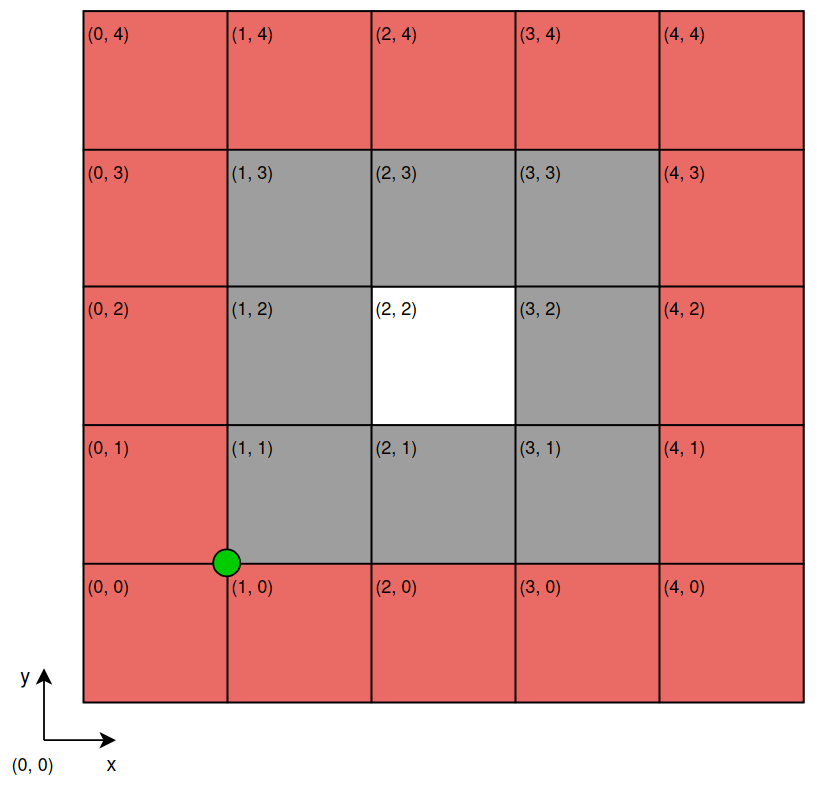
\includegraphics[width=0.8\linewidth]{images/modelo_del_mapa.png}
    \caption{Modelo del mapa}
    \label{fig:modelomapa}
\end{figure}
